%!TEX root = main.tex
\setcounter{chapter}{2}
\setcounter{section}{2}
\setcounter{theorem}{0}
\setcounter{equation}{0}

\lectureheader{161}{Calculus I}{Limits and limit laws}{\textit{Thomas' Calculus} \thesection}

\begin{mdframed}
\textbf{Idea of limit}:
Suppose that $\dom(f)$ contains points arbitrarily close to $c$.
We say that $f(x)$ approaches the \textbf{limit} $L$ as $x$ approaches $c$, and we write
\begin{equation*}
\lim_{x\to c}f(x) = L,
\end{equation*}
provided that $y$ can be made ``arbitrarily close" to $L$ by taking $x$ ``sufficiently close" (but not equal) to $c$ through $\dom(f)$.
\end{mdframed}

\begin{example}
Let $f(x) =\DS \frac{x^2-1}{x-1}$.
Observe that $f(1)$ is not defined.
Then compute $\DS\lim_{x\to 1} f(x)$.
\end{example}
\vfill

\newpage

\begin{remark}\,
\begin{itemize}
\item The limit does not care what is happening at $x=c$.
It only cares about what is happening on the approach to $x=c$.
\item Many limits can be evaluated by exploiting this fact.
\end{itemize}
\end{remark}

\begin{example}
Since the functions below agree everywhere except at $x=1$, we can say that
\begin{equation*}
\lim_{x\to 1}f(x) = \lim_{x\to 1}g(x) = \lim_{x\to 1}h(x) = 2.
\end{equation*}
\end{example}
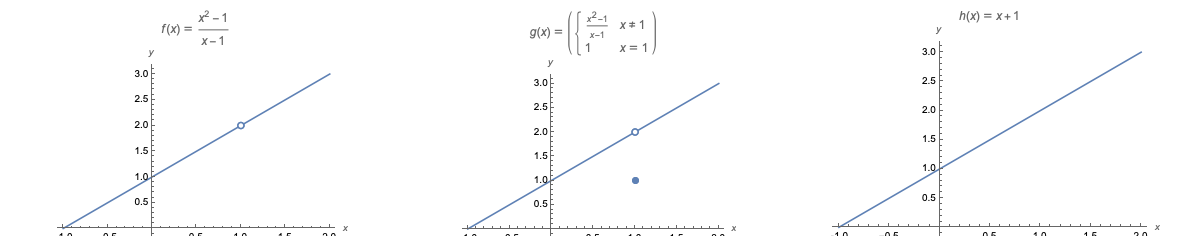
\includegraphics[width=6.75in]{img/limits-ex1}

\begin{example}
Why do the following not have limits as $x\to 0$?
\begin{enumerate}
\item $U(x) = \begin{cases} 0, & x<0\\ 1, & x\ge 0.\end{cases}$
\item $g(x) = \begin{cases} \frac{1}{x}, & x\ne 0\\ 0, &x=0.\end{cases}$
\item $f(x) = \begin{cases} 0,&x\le 0\\ \sin\frac{1}{x}, & x>0.\end{cases}$
\end{enumerate}
\end{example}
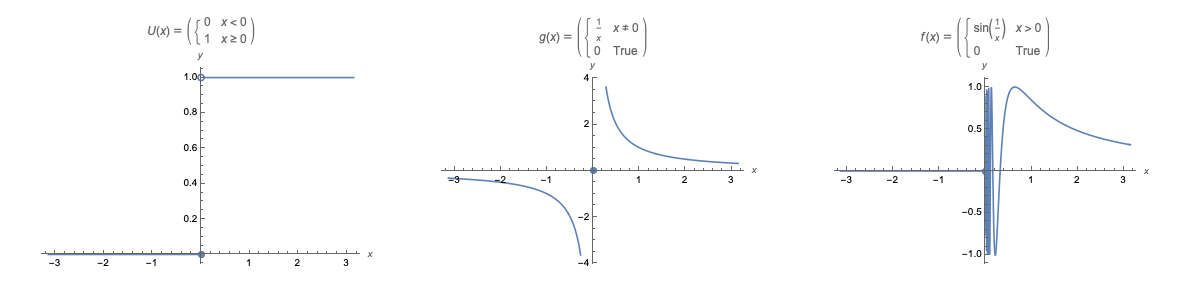
\includegraphics[width=6.75in]{img/limits-ex2}

\newpage

\begin{theorem}[Limit laws]
Let $f$ and $g$ be functions and $L,M,c\in\R$ so that
\begin{equation*}
\lim_{x\to c}f(x) = L\quad \text{and}\quad \lim_{x\to c}g(x) = M.
\end{equation*}
If $k\in\R$ and $n\in\N$, then
\begin{enumerate}
\item $\DS\lim_{x\to c}k = k$,
\item $\DS\lim_{x\to c}x = c$,
\item $\DS\lim_{x\to c}\big(f(x) \pm g(x)\big) = L\pm M$,
\item $\DS\lim_{x\to c}\big(f(x)g(x)\big) = L M$,
\item $\DS\lim_{x\to c}\frac{f(x)}{g(x)} = \frac{L}{M}$ if $M\ne 0$,
\item $\DS\lim_{x\to c}\big[f(x)\big]^n = L^n$, and
\item $\DS\lim_{x\to c}\sqrt[n]{f(x)} = L^{1/n}$,
\end{enumerate}
where in the last we assume that $f(x)\ge 0$ for $x$ near $c$ if $n$ is even.
\end{theorem}

\vfill

\begin{corollary}
If $p(x)$ and $q(x)$ are polynomials and $c\in\R$, then
\begin{enumerate}
\item $\DS\lim_{x\to c}p(x) = p(c)$, and
\item $\DS\lim_{x\to c}\frac{p(x)}{q(x)} = \frac{p(c)}{q(c)}$, assuming $q(c)\ne 0$.
\end{enumerate}
\end{corollary}
\vfill


\begin{example}
Evaluate the following.
\begin{enumerate}
\item $\DS\lim_{x\to 1}(x^3+4x^2-3)$
\vfill
\item $\DS\lim_{x\to 2}\frac{x^4+x^2-1}{x^2+5}$
\vfill
\item $\DS\lim_{x\to 3}\sqrt{4x^2-3}$
\vfill
\end{enumerate}
\end{example}

\newpage

\begin{itemize}
\item Later we will say that if $f$ is ``continuous" at $c$, then $\DS\lim_{x\to c}f(x) = f(c)$.
\item When $f$ is ``discontinuous" at $c$, simply plugging in $x=c$ will not work.
\item Sometimes we can evaluate the limit at a discontinuity by ``removing the discontinuity" using algebraic tricks.
\end{itemize}

\begin{example}
Evaluate the following.
\begin{enumerate}
\item $\DS\lim_{x\to 1}\frac{x^2+x-2}{x^2-x}$
\vfill
\item $\DS\lim_{x\to 0}\frac{x^2+x-2}{x^2-x}$
\vfill
\item $\DS\lim_{x\to 0}\frac{\sqrt{x^2+100}-10}{x^2}$
\vfill
\end{enumerate}
\end{example}

\newpage

\begin{theorem}[The squeeze/sandwich theorem]\,
\begin{enumerate}
\item Suppose that $g(x)\le f(x)\le h(x)$ for all $x$ in some open interval containing $c$, except possibly at $x=c$ itself.
\item Suppose $\DS\lim_{x\to c}g(x) = L = \lim_{x\to c}h(x)$.
\end{enumerate}
Then $\DS\lim_{x\to c}f(x) = L$.
\end{theorem}

\begin{example}
Evaluate the following.
\begin{enumerate}
\item $\DS\lim_{x\to 0}\sin x$
\vfill
\item $\DS\lim_{x\to 0}\cos x$
\vfill
\end{enumerate}
\end{example}

